\documentclass[xcolor=table]{beamer}
\usepackage[spanish]{babel}
\usepackage[utf8]{inputenc}
\usepackage{listings}
\usepackage[table]{xcolor}
\usepackage{multicol}
\usepackage{colortbl}
\mode<presentation> {
  \usetheme{Warsaw}
  %\beamerdefaultoverlayspecification{<+->} %Every new bullet includes \pause
}

\newcommand{\autor}{Pedro Pozuelo Rodríguez}
\newcommand{\titulo}{Reverse Proxy con capacidades de\\Firewall de aplicación web y aceleración TLS}
\newcommand{\profesor}{Ana del Valle Corrales Paredes}
\newcommand{\PFGID}{Pendiente}
\newcommand{\fechaversion}{\today}

\title[Reverse Proxy + WAF + aceleración TLS]{\titulo}
\author[\autor]{Alumno: \autor \and \and \and \and \and \and \and \and \and \and \and% Really crappy approach for getting authors in different lines:(
Directora: \profesor}
\institute{Universidad Europea\\Proyecto de Fin de Grado}
\date{\fechaversion}
\logo{
\includegraphics[height=1cm]{fig/universidad_logo}}

%\setbeamersize{text margin left=1cm, text margin right=1cm}

% Remove navigation icons
\beamertemplatenavigationsymbolsempty


\begin{document}
\AtBeginSection[] {
  \begin{frame}[shrink]
    \frametitle{\titulo}
    \tableofcontents[currentsection]
  \end{frame}
}

\begin{frame}
  \titlepage
\end{frame}

% Logo for the Titlepage
\logo{
\includegraphics[height=0.5cm]{fig/universidad_logo_notext}}

% Logo for all the other pages
\titlegraphic{
\includegraphics[width=2cm]{universidad_logo}\hspace*{4.75cm}~%
  
\includegraphics[width=2cm]{universidad_logo}
}

\chapter{Introducción}
\par En los últimos años, la mayoría de los ataques en Internet se realizan contra aplicaciones web, con lo que es cada vez más importante
contar con una solución que sea capaz de analizar el tráfico web y proteger dichas aplicaciones.
\par Desgraciadamente, no existe una aplicación completamente segura tal como afirma el adagio:

\say{La seguridad 100\% no existe.}

\par Con este punto de partida, y teniendo en cuenta el uso masivo que las aplicaciones hacen del Protocolo de transferencia de hipertexto (en adelante \acrshort{http}, de sus siglas en inglés\acrlong{http}) y del
Protocolo seguro de transferencia de hipertexto (en adelante \acrshort{https}, de sus siglas en inglés \acrlong{https}), es inmediato identificar porqué la mayoría de los ataques actuales se realizan contra aplicaciones publicadas a través de
estos protocolos.

\par Para protegerlas existen múltiples mecanismos de seguridad, desde herramientas que monitorizan el uso indebido de datos como el Software de prevención de pérdida de datos (en
adelante \acrshort{dlp}, de sus siglas en inglés \acrlong{dlp}), herramientas de red como son el firewall tradicional o herramientas más dirigidas como son los firewall de
aplicación web (en adelante \acrshort{waf}, de sus siglas en inglés, \acrlong{waf}).

\par En entornos con una gran infraestructura, que generen una facturación importante o con un alto riesgo, es habitual que se desplieguen las herramientas mencionadas y muchas otras, incluso herramientas redundantes siguiendo el principio de
\gls{DefensaProfundidad},  el cual aboga por desplegar múltiples sistemas de protección con el fin de que si uno falla otro pueda detener el ataque.
\par Pero, en entornos en los que los recursos son más limitados, no es viable desplegar todos los controles de seguridad que serían deseables. Por recursos no sólo se entiende
económicamente limitados como para invertir en tecnologías, si no también por personas con el tiempo, el conocimiento y la experiencia como para desplegar y mantenerlas.
\par En estos entornos es habitual que los controles de seguridad se limiten a un firewall de red o, si se dispone de algo más de presupuesto, un sistema de Gestión Unificada de
Amenazas (más conocido como \acrshort{utm}, de sus siglas en inglés\acrlong{utm}~\cite{wiki:utm}).
\par Estas soluciones, desgraciadamente, no son capaces de ofrecer una protección adecuada contra ataques en capa de aplicación. Por ejemplo, los firewall tradicionales son
capaces de analizar el tráfico de red en capa 3 del modelo TCP/IP (equivalente a las capas 3 y 4 del {\em modelo OSI\cite{osi}}). Esto implica que , cuando se publica un servicio web,
dichos firewalls permitirán todo el tráfico dirigido a estos servicios, con independencia de que se trate de una petición legítima, una petición incorrectamente formada o un ataque.
\par Para proteger estos servicios web adecuadamente es necesario disponer de tecnologías que entiendan analicen el tráfico en la capa de aplicación siguiendo la lógica propia del servicio a proteger, como los mencionados
WAF.

\par Otro aspecto que se debe tener en cuenta consiste en la migración constante que se está produciendo de forma generalizada de tráfico sin cifrar - también conocido como en texto plano - a tráfico cifrado HTTPS en el que se
encapsula el tráfico HTTP en un canal SSL/TLS. Históricamente se utilizaban múltiples herramientas perimetrales como son los sistema de detección de intrusiones (en adelante \acrshort{nids}, de sus siglas en inglés \acrlong{nids}) o los
mencionados firewalls. Desgraciadamente estas herramientas tradicionalmente no participan en la negociación SSL/TLS, por lo que no son capaces de descifrar el tráfico y no pueden analizar el contenido de las peticiones o sus respuestas. Estas
herramientas son, por lo tanto, cada vez menos efectivas a la hora de detectar y bloquear amenazas, pues carecen de la visibilidad adecuada en un gran porcentaje del tráfico.
\par Por último, se debe considerar otro cambio significativo que se está produciendo en estos últimos años: Cada vez es más habitual desplegar las aplicaciones en ~\gls{cloud} (o cloud, se utilizarán ambos términos indistintamente
debido a su uso extendido). En estos entornos se diluyen los conceptos de red perimetral o segmentación de red y es más complejo desplegar controles de seguridad perimetrales como los mencionados firewalls, NIDS o UTM. En estos entornos muchos
de los componentes de la infraestructura son transparentes para el cliente y no es posible desplegar mecanismos en estas capas.
\par A modo de referencia en la imagen {~\hyperref[fig:Responsabilidadescloud]{Responsabilidades compartidas en el cloud}} (fuente MR Informática~\cite{Responsabilidadescloud}) vemos como los únicos elementos sobre los que se mantiene el
control en los distintos modelos del cloud son la capa de aplicación y los datos (con la excepción del modelo de Software como un Servicio, en adelante \acrshort{saas}, de sus siglas en inglés \acrlong{saas}).
\begin{center}
  \label{fig:Responsabilidadescloud}
  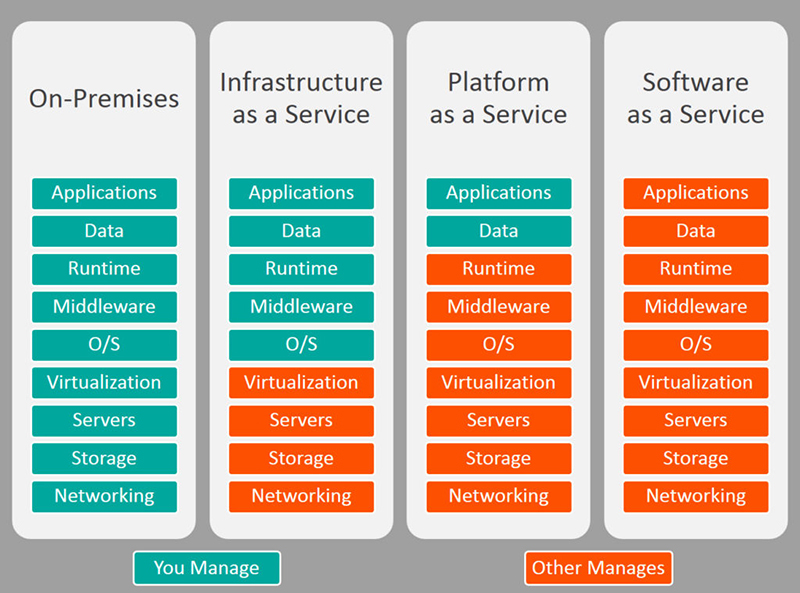
\includegraphics[width=0.7\textwidth]{fig/Responsabilidadescloud}
\end{center}

\par Es por lo tanto, cada vez más importante contar con herramientas que sean capaces de descifrar y analizar el tráfico HTTPS y, según se verá con más detalle en la sección de ~\nameref{subsec:estadoarte}, estas soluciones implican o bien un
desembolso económico significativo en el caso de las soluciones privativas o bien se despliegan como módulos de la propia aplicación web en las soluciones de {\em software libre\cite{softwarelibre}}.
\par En este segundo grupo las soluciones requieren un ejercicio de integración con las aplicaciones web y consumen recursos del servidor que pueden impactar en el rendimiento. Adicionalmente, para la implementación y configuración adecuada de
estos módulos se requiere de una persona con un conocimiento profundo de la seguridad de aplicaciones web que se mantenga informado de las últimas novedades del sector y que administre y actualice el entorno según se detectan nuevos ataques y
mecanismos paliativos.  Debido a estos factores y la complejidad que el WAF añade a la plataforma web, es habitual que cuando una plataforma web requiere de una actualización importante o una migración de tecnologías, el modulo de WAF se
desactive o elimine completamente.

\par Como respuesta a esta necesidad surge el presente proyecto, cuyo objetivo es construir una solución de software libre con capacidades de WAF, aceleración SSL/TLS, fácilmente desplegable y que minimice el esfuerzo y el impacto que dicha
solución tiene sobre la plataforma web actual o futura.

\chapter{Estado del arte}
\label{subsec:estadoarte}
\par Tal como se ha comentado en el capítulo anterior, un elemento clave para proteger las aplicaciones web es el WAF.

\par En primer lugar se ha procedido a realizar una análisis comparativo de las diferentes soluciones WAF disponibles en el mercado. Para ello, se ha utilizado el documento de buenas prácticas de OWASP\cite{owaspbestpractices} como referencia.
\par forma específica, el criterio seguido es que la solución debe ser capaz de proteger la plataforma web implementando una mayoría de los controles de seguridad (referenciados como {\em Countermeasure} en la página de OWASP\cite[apartado A3.2]{owaspbestpractices}).

\par Dentro de las soluciones disponibles, podemos distinguir principalmente entre soluciones privativas y soluciones de software libre. Este
criterio no se circunscribe exclusivamente al modelo de licencias si no que está íntimamente ligado al coste asociado tal como veremos.

\section{Soluciones WAF privativas}
\par Las soluciones de WAF privativas se caracterizan por emplear un modelo de {\em licenciamiento privativo\cite{privativo}}. Se trata de
soluciones con un elevado coste y con la imposibilidad de acceder al código o modificarlo. Así mismo, ofrecen una serie de funcionalidades
adicionales y una mayor capacidad de procesamiento.
\par Existen dos arquitecturas principales en este tipo de WAF:
\par Por un lado tenemos modelos WAF desplegados en las instalaciones del fabricante y gestionados por él. Este tipo de soluciones suelen estás
alojadas en el Cloud (en el modelo de distribución de software conocido como {\em software como servicio} (en adelante \acrshort{saas}, de sus
siglas en inglés, \acrlong{saas}).
\par En segundo lugar, tenemos WAF de tipo appliance o máquina virtual. Se trata de máquinas dedicadas en las que el software requiere de una
máquina específica proporcionada por el fabricante. Si bien hardware y software se adquieren conjuntamente, es posible acceder a nuevas
funcionalidades adquiriendo nuevas licencias.

\subsection{Soluciones WAF SaaS}
\par Dentro de las soluciones WAF SaaS, destacan y se han analizado {\em Cloud Web Application Firewall} \cite{cloudflarewaf} de Cloudflare\cite{cloudflare} ({\em Cloudflare} en adelante), {\em Kona WAF\cite{kona}} de {\em Akamai\cite{akamai}} e {\em Incapsula\cite{Incapsula}}.
\par Habitualmente, estos proveedores no se limitan a ofrecer servicios WAF, pues por su infraestructura permite añadir funcionalidades adicionales como son las siguientes.
\begin{itemize}
  \item Red de distribución de contenidos (en adelante \acrshort{cdn}, de sus siglas en inglés, \acrlong{cdn}).
  \item Protección contra ataques de denegación de servicio (en adelante \acrshort{dos}, de sus siglas en inglés, \acrlong{dos}) en capa de
    aplicación.
  \item Habilitar el caché de contenido estático.
  \item Suscripción a listas de reputación de IP, dominios o URL.
  \item Bloqueo de bots maliciosos.
  \item Sistema de creación de informes.
\end{itemize}
\par De hecho, la funcionalidad CDN es el servicio mínimo que se puede contratar a Akamai y Cloudflare; pues es su nicho mercado y su producto
principal, siendo el servicio WAF una funcionalidad que ofrecen a sus cliente para dar un valor añadido. Incapsula, por el contrario, proviene
de soluciones WAF tipo appliance y su modelo de negocio está más enfocado a estos servicios.
\par Uno de las principales características que comparten estos proveedores es el modelo de negocio. En todos los casos el coste está asociado
al volumen de tráfico que se genere, ya sea en caudal de datos (en adelante \gls{throughput}), como es el caso de Incapsula, o por volumen mensual de datos en el caso de Akamai y Cloudflare.

\subsubsection{Modo de licenciamiento y coste}
\label{subsec:wafsaaslic}
\par En la mayoría de las soluciones no existe un precio oficial de mercado proporcionado por los proveedores. En estos casos se ha optado por
incluir referencias externas con el fin de disponer información del coste aproximado de estas soluciones.
\par A modo de referencia, se puede consultar los precios de Akamai y Cloudflare en la {~\hyperref[tab:precioscdn]{tabla de precios CDN}}.
Estos precios se corresponden con sus servicios de CDN y podrá ser superior si se añaden funcionalidades como WAF. Adicionalmente, se debe
tener en cuenta que se trata de precios estimativos proporcionados por terceros, pues en el caso de Akamai la lista de precios no es pública y
ofrecen un coste ajustado a cada cliente.
\begin{table}[h!]
  \centering
  \label{tab:precioscdn}
  \begin{tabular}{rrr}
     &
    \multicolumn{1}{c}{\textbf{Akamai CDN}} &
    \multicolumn{1}{c}{\textbf{CloudFlare CDN}} \\
    \hline \hline
    6 TB plan   & 900  USD al mes aprox.  & 750   USD al mes aprox. \\
    \hline
    25 TB plan  & 2800 USD al mes aprox.  & 2800  USD al mes aprox. \\
    \hline
    50 TB plan  & 5500 USD al mes aprox.  & 5000+ USD al mes aprox. \\
    \hline
    100 TB plan & 8000 USD al mes aprox.  & 5000+ USD al mes aprox. \\
    \hline
  \end{tabular}
  \caption{Precios de CDN\cite{cdnprices} (consultado en abril de 2019)}
\end{table}

\par En el caso de Incapsula, su solución más económica - el plan {\em PRO} -  tiene un coste de 59 USD por web al mes\cite{incapsulaprices}.
Dicha solución soporta SSL de manera limitada y es necesario contratar un plan superior en caso de que se requiera dar servicio a clientes que
no soporten la extensión TLS \acrshort{SNI} o se requieran certificados con validación extendida (en adelante \acrshort{ev}, de sus siglas en
inglés, \acrlong{ev}). En esta situación habría que contratar el plan {\em business} que tiene un coste de 299 USD por web al
mes\cite{incapsulaprices}.

\subsubsection{Implementación y operación}
\par Independientemente de la solución, grosso modo estos son los pasos a realizar para implantar este tipo de soluciones:
\begin{enumerate}
  \item Cambio en la gestión de certificados SSL.
    \par Dado que la mayoría de las aplicaciones web deben soportar SSL, es necesario generar nuevos certificados para que el proveedor pueda
    publicar los servicios web de manera confiable. En la mayoría de los casos el fabricante será responsable del mantenimiento y la operación
    de dichos certificados.
  \item Preparación de un entorno de pruebas - {\em staging} - en el que se puedan probar las aplicaciones web de manera interna sin impactar
    a los clientes. Para ello, habitualmente, se redireccionan los dominios a probar en el fichero {\em hosts} de la máquina cliente.
  \item Cambio del direccionamiento DNS.
    \par Una ya se ha validado que la solución web y el WAF funcionan adecuadamente, se procede a cambiar el direccionamiento ofrecido a nivel
    DNS para que los clientes se conecten a la plataforma WAF en lugar de a la aplicación web.
\end{enumerate}

\par La operación de estas plataformas es realizada por el proveedor, por lo que como clientes no necesitamos disponer del conocimiento o el
tiempo necesario para mantener o actualizar la plataforma WAF.

\subsubsection{Ventajas}
\par Una de las principales ventajas que tiene este tipo de soluciones consiste en su independencia respecto a la infraestructura de la
aplicación web.
\par Esta independencia nos permite realizar cambios en cualquier de las soluciones - WAF o plataforma Web - sin que afecte a la otra. Ya sean
cambios en la operación diaria, migraciones de software o rediseño de la arquitectura.
\par La mencionada independencia no se limita a independencia tecnológica; el hecho de que el WAF y la plataforma web sean completamente
independientes también permite asignar roles independientes a cada entorno, lo cual permite implementar seguridad basada en roles (en adelante
\acrshort{rbac}, de sus siglas en inglés, \acrlong{rbac}). Esto no sólo nos permite mejorar la seguridad del entorno, si no que además evita
que el desarrollador web o el administrador de la plataforma web tenga que conocer en detalle la configuración del WAF y viceversa.

\par Por otro lado, este tipo de soluciones son las muy sencillas de implementar, tal como se ha visto en la sección anterior.
\par Otra ventaja radica en la aplicación de nuevas reglas de seguridad de forma transparente para el cliente. No necesitaremos dar seguimiento
a las últimas vulnerabilidades web que se publican o idear qué reglas o firmas son necesarias, pues el proveedor se hará cargo de su
implementación y mantenimiento.
\par Las soluciones WAF SaaS también nos permiten contratar diversas modalidades de soporte que garanticen respuesta 24/7 en caso de que se
produzca un incidente con el servicio.
\par Por último, nos podemos beneficiar de las funcionalidades adicionales ya mencionadas para mejorar el estado de la seguridad de nuestra
plataforma o mejorar la experiencia del usuario.


\subsubsection{Desventajas}
\par Una de las principales desventajas radica en el coste económico. Este tipo de soluciones tienen un elevado coste. Esto implica que este tipo de WAF sólo son viables económicamente en portales que generen un beneficio económico importante o aquellos en los que la empresa/entidad responsable de la aplicación pueda asumir su inversión.
\par Aunque este tipo de soluciones disponen de modalidades relativamente económicas (ver ~\nameref{subsec:wafsaaslic}), lo cierto es que estas soluciones
están muy limitadas y es necesario contratar funcionalidades adicionales en la mayoría de los casos. Es un modelo económico muy dirigido a las
ofertas personalizadas y suele ser habitual requerir el modelo de licenciamiento {\em Enterprise} junto con ciertas licencias adicionales, lo
cual encarece todavía más el servicio.
\par En cualquier caso, este tipo de soluciones no están al alcance de pequeñas o medianas empresas o de particulares.

\par Otra desventaja que tienen este tipo de soluciones consiste en la pocas posibilidades que tenemos de personalizar las reglas o las firmas
a nuestras necesidades. La arquitectura de este tipo de plataformas SaaS consiste en que múltiples clientes comparten la misma plataforma, para
lo cual el proveedor requiere mantener un sistema homogéneo para todos los clientes y esto evita que se pueda personalizar el WAF según
nuestras necesidades. A modo de ejemplo, en los servicios estándar de este tipo de soluciones no podremos configurar reglas para filtrar las
cabeceras HTTP o los parámetros de tipo query en las URL si nuestra aplicación utilizada {\em Path Parameters} o {\em URL Routing}, lo que
dejaría expuesta la aplicación web a ataques de inyección de código.


\subsection{Soluciones WAF tipo Appliance}
\par Otra modalidad de soluciones WAF son los de tipo appliance. Dentro de las opciones disponibles en el mercado se han analizado {\em Imperva
WAF Gateway\cite{imperva}} ({\em Imperva} en adelante) y {\em Fortiweb\cite{fortiweb}} de la empresa {\em Fortinet\cite{fortinet}}.
\par El modelo de negocio tradicional consiste en adquirir máquina física junto con un paquete de licencias, aunque en los últimos años se han
incorporado soluciones virtuales en los catálogos de los principales proveedores de Cloud.
\par Al igual que sucede con las soluciones SaaS, los proveedores de este tipo de WAF también incluyen mecanismos de seguridad adicionales que
no son propiamente funcionalidades WAF. Si bien estas funcionalidades dependen en gran medida del proveedor, a continuación se enumeran algunas
de las más interesantes:
\begin{itemize}
  \item Crear perfiles de las aplicaciones web y filtrar las peticiones web en función de los parámetros permitidos.
  \item Parcheo virtual de vulnerabilidades mediante la integración del WAF con programas de escaneo de vulnerabilidades.
  \item Suscripción a listas de reputación de IP, dominios o URL.
  \item Aceleración TLS.
    \par Dado que el dispositivo suele estar en la misma red que la aplicación web, es posible que el WAF realice el descifrado del tráfico
    SSL/TLS y envíe el tráfico sin cifrar a la aplicación web, lo que permite liberar los recursos asignados al cifrado y descifrado en la
    aplicación web.
  \item Bloqueo de bots maliciosos.
  \item Sistema de creación de informes.
  \item Antivirus.
\end{itemize}

\subsubsection{Modo de licenciamiento y coste}
\par Al igual que sucede con las soluciones SaaS, en las soluciones appliance los proveedores no publican abiertamente el coste que tienen sus
productos y optan por realizar presupuestos personalizados dependiendo de las necesidades de cada cliente. Al igual que en el análisis del
modelo SaaS se ha optado por incluir referencias externas con el fin de mostrar el coste que tienen este tipo de soluciones.

\par En el caso de Imperva, su oferta está enfocada a soluciones WAF y firewall de base de datos (en adelante \acrshort{dbf}, de sus siglas en
inglés, \acrlong{dbf}). Se trata de la misma compañía que ha desarrollado y comercializa Incapsula, siendo ésta la alternativa SaaS a Imperva.
\par Imperva ofrece diversos modelos de appliances según el throughput que son capaces de gestionar, desde 500 Mbps en el modelo más
básico - X2010 o X2020 - hasta los 10 Gbps en el modelo X10K. \par El coste del appliance de 500 Mbps es de 4200 USD (según \cite{impervacost1} y
\cite{impervacost2}), a lo que hay que sumar el coste anual de licencias y mantenimiento. La licencia necesaria para este modelo tiene un
coste que puede ir desde 4800 USD\cite{impervacost3} hasta 9600 USD\cite{impervacost4}. Por lo tanto, la opción más económica requiere una
inversión inicial de 9000 USD y un coste anual mínimo de 4800 USD.

\par En el caso de que la plataforma web esté alojada en el Cloud (por ejemplo AWS), la opción más económica ofrecida por Imperva tiene un
coste mínimo de 8927 USD anuales para una instancia con capacidad de hasta 100 Mbps\cite{impervaawscost1} o 21567 USD por año para el equivalente de
la opción appliance de 500 Mbps\cite{impervaawscost2}.

\par Otra solución appliance que se ha analizado es Fortiweb. Si bien sigue un modelo de negocio similar a Imperva, dispone de modelos más
económicos. En la {~\hyperref[tab:preciosfortiweb]{tabla de precios Fortiweb}} se recogen los modelos appliance más económicos ofrecidos por
Fortinet.

\begin{table}[h!]
  \centering
  \label{tab:preciosfortiweb}
  \begin{tabular}{|r|r|r|r|r|}
    \hline
    Modelo                  & Throughput & Coste de appliance             & Coste licencia básica          & Coste total  \\
    \hline
    \textbf{FortiWeb-100D}  & 25 Mbps    & 5034 USD\cite{fortiwebcost1}  & 755 USD\cite{fortiwebcost1}   &  5789 USD    \\
    \hline
    \textbf{FortiWeb-400D}  & 100 Mbps   & 9194 USD\cite{fortiwebcost2}  & 1572 USD\cite{fortiwebcost2}  & 10766 USD    \\
    \hline
    \textbf{FortiWeb-600D}  & 250 Mbps   & 14000 USD\cite{fortiwebcost3} & 2100  USD\cite{fortiwebcost3} & 16100 USD    \\
    \hline
  \end{tabular}
  \caption{Precios de Fortiweb}
\end{table}
\par La solución AWS de Fortiweb tiene un coste de 5374 USD\cite{fortiwebcost4} al año.

\subsubsection{Implementación y operación}
\par La implementación de las soluciones tipo appliance es más compleja que en el modelo SaaS debido a que el WAF será parte de nuestra
arquitectura y es necesario analizarla y adaptarla con el fin de incluir este nuevo elemento.
\par Los pasos que se deben realizar para implantar un WAF de tipo appliance en una arquitectura son los siguientes:

\begin{enumerate}
  \item Evaluar la arquitectura actual e identificar los potenciales puntos en los que se podría desplegar el WAF.
    \par Algunos de los punto de conexión donde se suelen desplegar WAF de este tipo son inmediatamente después del firewall red o
    inmediatamente antes de los balanceadores de carga de aplicación, pero puede variar significativamente según la arquitectura. Especialmente se debe
    tener en cuenta los siguientes elementos:
    \begin{itemize}
      \item Tolerancia frente a fallos (en adelante {\em failover}).
      \item Tipo de enrutamiento: estático o dinámico, unicast o multicast, etc.
      \item Sistemas distribuidos o redundantes.
      \item Balanceadores de red o de aplicación.
      \item Volumen de tráfico en los distintos puntos de red a evaluar.
        \par Por ejemplo, si se instala el WAF en el punto de entrada de una DMZ, el appliance debe ser capaz de gestionar el throughput
        agregado de todos los servicios publicados en dicha DMZ. Sin embargo, si se instala inmediatamente antes de una aplicación web, el WAF
        sólo debe analizar el tráfico de dicha aplicación. Por contra, si se despliega una nueva aplicación web es posible que ésta no esté
        protegida por el WAF.
      \item Lógica de la aplicación web.
        \par A modo de ejemplo, en una arquitectura en la que se disponga de un  servidor web para servir contenido estático, es posible
        configurar el WAF para que no acepte el paso de parámetros o que sólo proteja el servidor web de contenido dinámico si se decide
        aceptar el riesgo asociado.
      \item Aplicación alojada en un único centro de datos (en adelante CPD) o en varios.
    \end{itemize}

  \item Analizar dichos puntos y evaluar el modo de despliegue en el que se desplegará el WAF. Los modos más comunes son modo transparente, en
    el que el WAF no participa en las capas 3 a 7 del modelo OSI, o como proxy web explícito, en cuyo caso el WAF participa en las capas 3 y 4
    y opcionalmente en la capa de aplicación.
  \item Evaluar el impacto que este cambio tendrá en el desempeño de la aplicación web, entre otros se debe evaluar la latencia que añade a la
    red y a la aplicación o cómo afecta al throughput que deben soportar los distintos componentes.
  \item Adaptar el diseño de red incluyendo los nuevos elementos.
  \item Elegir el o los modelos de appliance que mejor cumple las necesidades del nuevo diseño.
  \item Desplegar los nuevos elementos. Típicamente este punto comprende las siguientes actividades:
    \begin{enumerate}
      \item Instalación de la solución en el bastidor del CPD (en adelante rack).
      \item Conexión y configuración de las interfaces de gestión y de los elementos de red necesarios.
      \item Instalación de los certificados SSL y configuración inicial de las funcionalidades WAF.
      \item Preparación de un entorno de pruebas de forma similar a la indicada para WAF de tipo SaaS.
      \item Cambio del direccionamiento de DNS o de IP según proceda.
        \par Una ya se ha validado que la solución web y el WAF funcionan adecuadamente, se procede a cambiar el direccionamiento ofrecido a nivel
        de red para que el tráfico de la aplicación web se enrute a través del WAF.
    \end{enumerate}
\end{enumerate}

\par Si se comparan estas actividades con las equivalente de la solución WAF SaaS, esta solución es más compleja de desplegar y se deben tener
en cuenta más factores. Esto es así debido a que al elegir esta solución se debe modificar la arquitectura de red y debemos tener en cuenta
cómo WAF va a impactar a la plataforma web.
\par Por otro lado, dado que la administración y mantenimiento no están delegados en una empresa externa, debemos disponer de las personas
adecuadas - con conocimiento, experiencia y tiempo - para administrar y operar el WAF.

\subsubsection{Ventajas}
\par Las soluciones WAF de tipo appliance son más personalizables que las soluciones WAF SaaS. Esto es así debido a que disponemos de unos
dispositivos dedicados para nuestra plataforma web, y por lo tanto podemos crear reglas específicas que se adapten a nuestras necesidades.
\par Estas soluciones también cuenta como ventaja que toda la información está en nuestras instalaciones, lo cual nos permite tener mayor
control de la información y puede simplificar el cumplimiento de ciertas regulaciones, como son el reglamento europeo \acrshort{rgdp} o el
Estándar de Seguridad de Datos para la Industria de Tarjeta de Pago (en adelante \acrshort{pcidss}, de sus siglas en inglés, \acrlong{pcidss}).
\par Una ventaja que comparten con las soluciones SaaS es su independencia del software utilizado en la plataforma web. Esto es así debido a
que se despliegan como un elemento perimetral y no está conectado con la plataforma web a nivel de aplicación.
\par Igualmente, comparten las ventajas de independencia operacional; aunque en el caso de los WAF de appliance esta independencia es
prácticamente obligatoria debido a que requiere un mayor conocimiento especializado tal como se verá en la siguiente sección.
\par Al igual que los WAF SaaS, en este tipo de soluciones requiere un servicio de mantenimiento o de suscripción; esto permite que no sea
necesario mantenerse al día de las últimas vulnerabilidades y podamos abstraernos parcialmente de cómo proteger la plataforma, pues lo
proveedores mantienen las reglas actualizadas como parte del servicio contratado.
\par Por último, las soluciones WAF de tipo appliance también nos permiten añadir algunos de los mecanismos de seguridad que no son propiamente
de WAF que se han comentado anteriormente.

\subsubsection{Desventajas}
\par Tal como se ha anticipado, implementar y administrar este tipo de soluciones requiere de ciertos conocimientos en materia de seguridad,
tanto acerca de las técnicas ofensivas más frecuentes, como los mecanismos necesarios para proteger la infraestructura.
\par Por otro lado, la capacidad de crear nuevas reglas en este tipo de entornos es limitada. Si bien se menciona como ventaja que estos WAF
permiten mayor versatilidad que las soluciones SaaS, hay que tener en cuenta que todas las soluciones de este tipo hacen uso de licencias de
software privativas, con las restricciones que este tipo de licencias implica:  No es posible acceder al código fuente o modificarlo para
implantar nuevas funcionalidades o solucionar fallos y el ciclo de vida del appliance es el que el fabricante impone.
\par Este problema se agrava en las soluciones de tipo appliance debido a que no es infrecuente que el fabricante imponga la renovación de
hardware o software de forma agresiva y nos veamos obligados a realizar inversiones adicionales no planificadas.

\par Otra desventaja de este tipo de soluciones es su elevado coste económico. Si bien el coste recurrente suele ser inferior a las soluciones
SaaS equivalentes, sigue siendo un coste elevado; por otro lado, las soluciones WAF de tipo appliance requieren la compra de los dispositivos,
lo que supone un mayor coste de inversión inicial que en las soluciones SaaS.
\par Al igual que sucede con las soluciones SaaS, este tipo de soluciones no están al alcance de pequeñas o medianas empresas o de
particulares.

\section{Soluciones WAF de software libre}
\par Dentro de las soluciones WAF de software libre, se han evaluado las siguientes:
\begin{itemize}
  \item IronBee\cite{IronBee}.
  \item WebCastellum\cite{WebCastellum}.
  \item RAPTOR\cite{raptor}.
  \item NAXSI\cite{NAXSI}.
  \item OpenWAF\cite{openwaf}.
  \item FreeWAF\cite{freewaf}.
  \item Shadow Daemon\cite{ShadowDaemon}.
  \item AQTRONiX WebKnight\cite{WebKnight}.
  \item Vulture\cite{vulture}.
  \item ModSecurity \cite{modsecurity}.
\end{itemize}

\par Entre ellas destaca ModSecurity por ser la solución de software libre más extendida y activa de la comunidad e implementa un número
significativo de los controles de seguridad deseables en un WAF.
\par También destacan OpenWAF y FreeWAF (también conocido como {\em lua-resty-waf}) debido a que tienen un planteamiento y unas
funcionalidades muy interesantes.
\par Éstas y las demás soluciones se evaluarán en la posterior fase de análisis.


\subsubsection{Modo de licenciamiento y coste}
En la {~\hyperref[tab:waflibre]{tabla resumen de WAF de software libre}} podemos comparar las diferentes soluciones:

\begin{table}[h!]
  \centering
  \label{tab:waflibre}
  \begin{tabular}{llll}
    \hline
     Solución             & Licencia                        & Coste                           & Soporte                         \\
    \hline
     IronBee              & Apache License 2.0              & Gratuito                        & No                              \\
     WebCastellum					& Eclipse Public License          & Gratuito                        & No                              \\
     RAPTOR					      & GNU GPL 2.0                     & Gratuito                        & No                              \\
     NAXSI					      & GNU GPL 3.0                     & Gratuito                        & Comunidad                       \\
     OpenWAF					    & BSD license                     & Gratuito                        & Comunidad                       \\
     FreeWAF					    & GNU GPL 3.0                     & Gratuito                        & Comunidad                       \\
     Shadow Daemon				& GNU GPL 2.0                     & Gratuito                        & Comunidad                       \\
     WebKnight		        & GNU GPL                         & 145 USD / año                   & Proveedor                       \\
     Vulture					    & No se especifica                & Gratuito                        & Proveedor(de pago)              \\
     ModSecurity 					& Apache License 2.0              & Gratuito y de pago\hyperlink{modlic}{*}  & Comunidad o Proveedor  \\
    \hline
  \end{tabular}
  \caption{Modos de licenciamiento y costes de WAF de software libre}
\end{table}

\par \hypertarget{modlic}{*} Modsecurity ofrece la solución WAF de forma gratuita, que cuenta con soporte por parte de la
comunidad, y una versión de pago por 495 USD al año que ofrece soporte por parte de Trustware\cite{trustware} y un conjunto mayor de reglas
\cite{modsecuritysupport}.

\subsubsection{Implementación y operación}
\par Las soluciones WAF de software libre se implementan, en la mayoría de los casos, como módulos adicionales al servidor de aplicación web,
ya sea Apache HTTP Server\cite{apache} (en adelante, Apache), Nginx\cite{nginx}, Internet Information Services\cite{iis}, etc.
\par Esto implica que el WAF debe ejecutarse como parte del servicio web y su configuración y operación depende del administrador de la
plataforma web.
\par Si en los WAF de tipo appliance se ha visto que las tareas de implantación tienen cierta complejidad en lo relativo a analizar la
plataforma web desde un punto de vista de red, en el caso de los WAF que se ejecutan como parte del servicio web la complejidad radica en que
el WAF debe integrarse dentro de la plataforma web.
\par Este tipo de WAF requiere que se revise el dimensionamiento de la plataforma web debido a que consumen recursos del servidor y puede
afectar a su rendimiento.

\par Estas son las tareas que se deben abordar de forma genérica a la hora de implantar un WAF de software libre:
\begin{enumerate}
  \item Evaluar la plataforma web actual e identificar qué soluciones WAF son compatibles con el servicio web.
  \item Desplegar un un entorno de pruebas equivalente a la plataforma web actual o prueba de concepto (en adelante \acrshort{poc}, de sus
    siglas en inglés, \acrlong{poc}).
  \item Desplegar el WAF en el entorno de pruebas.
  \item Realizar pruebas exhaustivas sobre el nuevo entorno, especialmente pruebas funcionales y de rendimiento.
  \item Evaluar el impacto del WAF, entre otros se debe evaluar errores en la lógica de aplicación, latencia que añade, aumento en el consumo
    de recursos o cómo afecta al throughput soportado por la plataforma.
    \par Tradicionalmente este punto y el anterior se deberán ejecutar de forma reiterativa hasta que los resultados sean concluyentes y la
    nueva configuración se considere suficientemente robusta como para desplegarla en producción.
  \item Desplegar el WAF en el entorno de producción (si la plataforma lo permite, se recomienda realizar el despliegue de forma escalonada) y
    realizar un conjunto de pruebas similar a las realizadas en el entorno de pruebas.
\end{enumerate}

\par Aunque en este tipo de soluciones se han enumerado menos pasos que en las soluciones anteriores, esto es debido a que las tareas dependen
en gran medida del software y la plataforma elegidos, por lo que las actividades se han identificado de forma más general.

\subsubsection{Ventajas}
\par Los WAF de software libre son más económicos que las alternativas privativas. Si bien es cierto que esto no quiere decir que sean gratis,
pues requieren personas que los administren y consumen una serie de recursos de la plataforma web.
\par Pero, aun eligiendo alguna de las opciones de pago y con soporte como por ejemplo ModSecurity, el coste en licencias es muy inferior a las
otros modelos privativos.
\par Debido al tipo de licenciamiento, estas soluciones se distribuyen como software libre, con todas las ventajas inherentes a este
tipo de software entre las que destaca desde un punto de vista funcional el acceso al código fuente y la capacidad de modificarlo de acuerdo a
nuestras necesidades entre otras. Está fuera del alcance del documento evaluar las ventajas generales del software libre frente a otro tipo de
licencias.
\par No en todos los casos, pero en la mayoría de las soluciones analizadas el equipo de desarrollo es un conjunto de individuos pertenecientes
a distintos ámbitos o empresas, por lo que se elimina la estricta dependencia del proveedor. Si bien este modelo tiene sus ventajas e
inconvenientes, lo cierto es que se elimina la dependencia de realizar una migración del software si se considera conveniente (por ejemplo,
para alinear dicha migración según una planificación propia en lugar de una planificación impuesta).
\par Se puede pues decir que estas soluciones son más adaptables a las necesidades específicas de cada entorno.

\subsubsection{Desventajas}
\par Este tipo de soluciones son más difíciles de implementar y de mantener. El hecho de que estén integradas como parte de la plataforma web
hace que sea complejo diferenciar los roles del administrador de la plataforma web del administrador del WAF. Por lo tanto, la misma persona
debe tener conocimiento de ambas plataformas y ambos campos del conocimiento, lo cual no es común y puede provocar en errores de configuración
de alguna de las plataformas.
\par Precisamente debido a la gran dependencia existente entre el software WAF y de la plataforma web, es necesario analizar en detalle las
configuraciones y las reglas que se habilitarán, pues el proceso de depuración de errores es más complejo y los fallos son más difíciles de
identificar y solucionar.
\par Las actividades de actualización de componentes y migraciones de software son así mismo más complejas, pues se deben actualizar o migrar
ambas plataformas conjuntamente.
\par Por otro lado, el soporte en este tipo de soluciones puede ser de menor calidad que en las alternativas privativas. Al fin y al cabo en
muchos casos el soporte depende de la comunidad y si se elige un WAF que tenga una comunidad reducida, es probable que no se obtenga una
respuesta inmediata. Por supuesto, si se elige una solución con soporte o se contrata un servicio de consultoría, se puede paliar esta
desventaja. Si se trata de un entorno de producción en el que el tiempo de caída del servicio es crítico, se recomienda contratar algún
servicio de soporte o consultoría.


\section{Solucion}
\subsection{Objetivo}
\begin{frame}[shrink]
  \frametitle{Objetivo}
  Como respuesta a la situación actual, se define el siguiente objetivo:
  \begin{block}{Objetivo}
    Construir una solución de software libre con capacidades de WAF y aceleración SSL/TLS, que sea  fácilmente desplegable y que minimice el esfuerzo y el impacto que dicha
    solución tiene sobre la plataforma web actual o futura.
    \par También debe ser fácilmente adaptable a diferentes necesidades y entornos.
  \end{block}
\end{frame}

\subsection{Diseño}
\begin{frame}[shrink]
  \frametitle{Diseño}
  \begin{figure}
    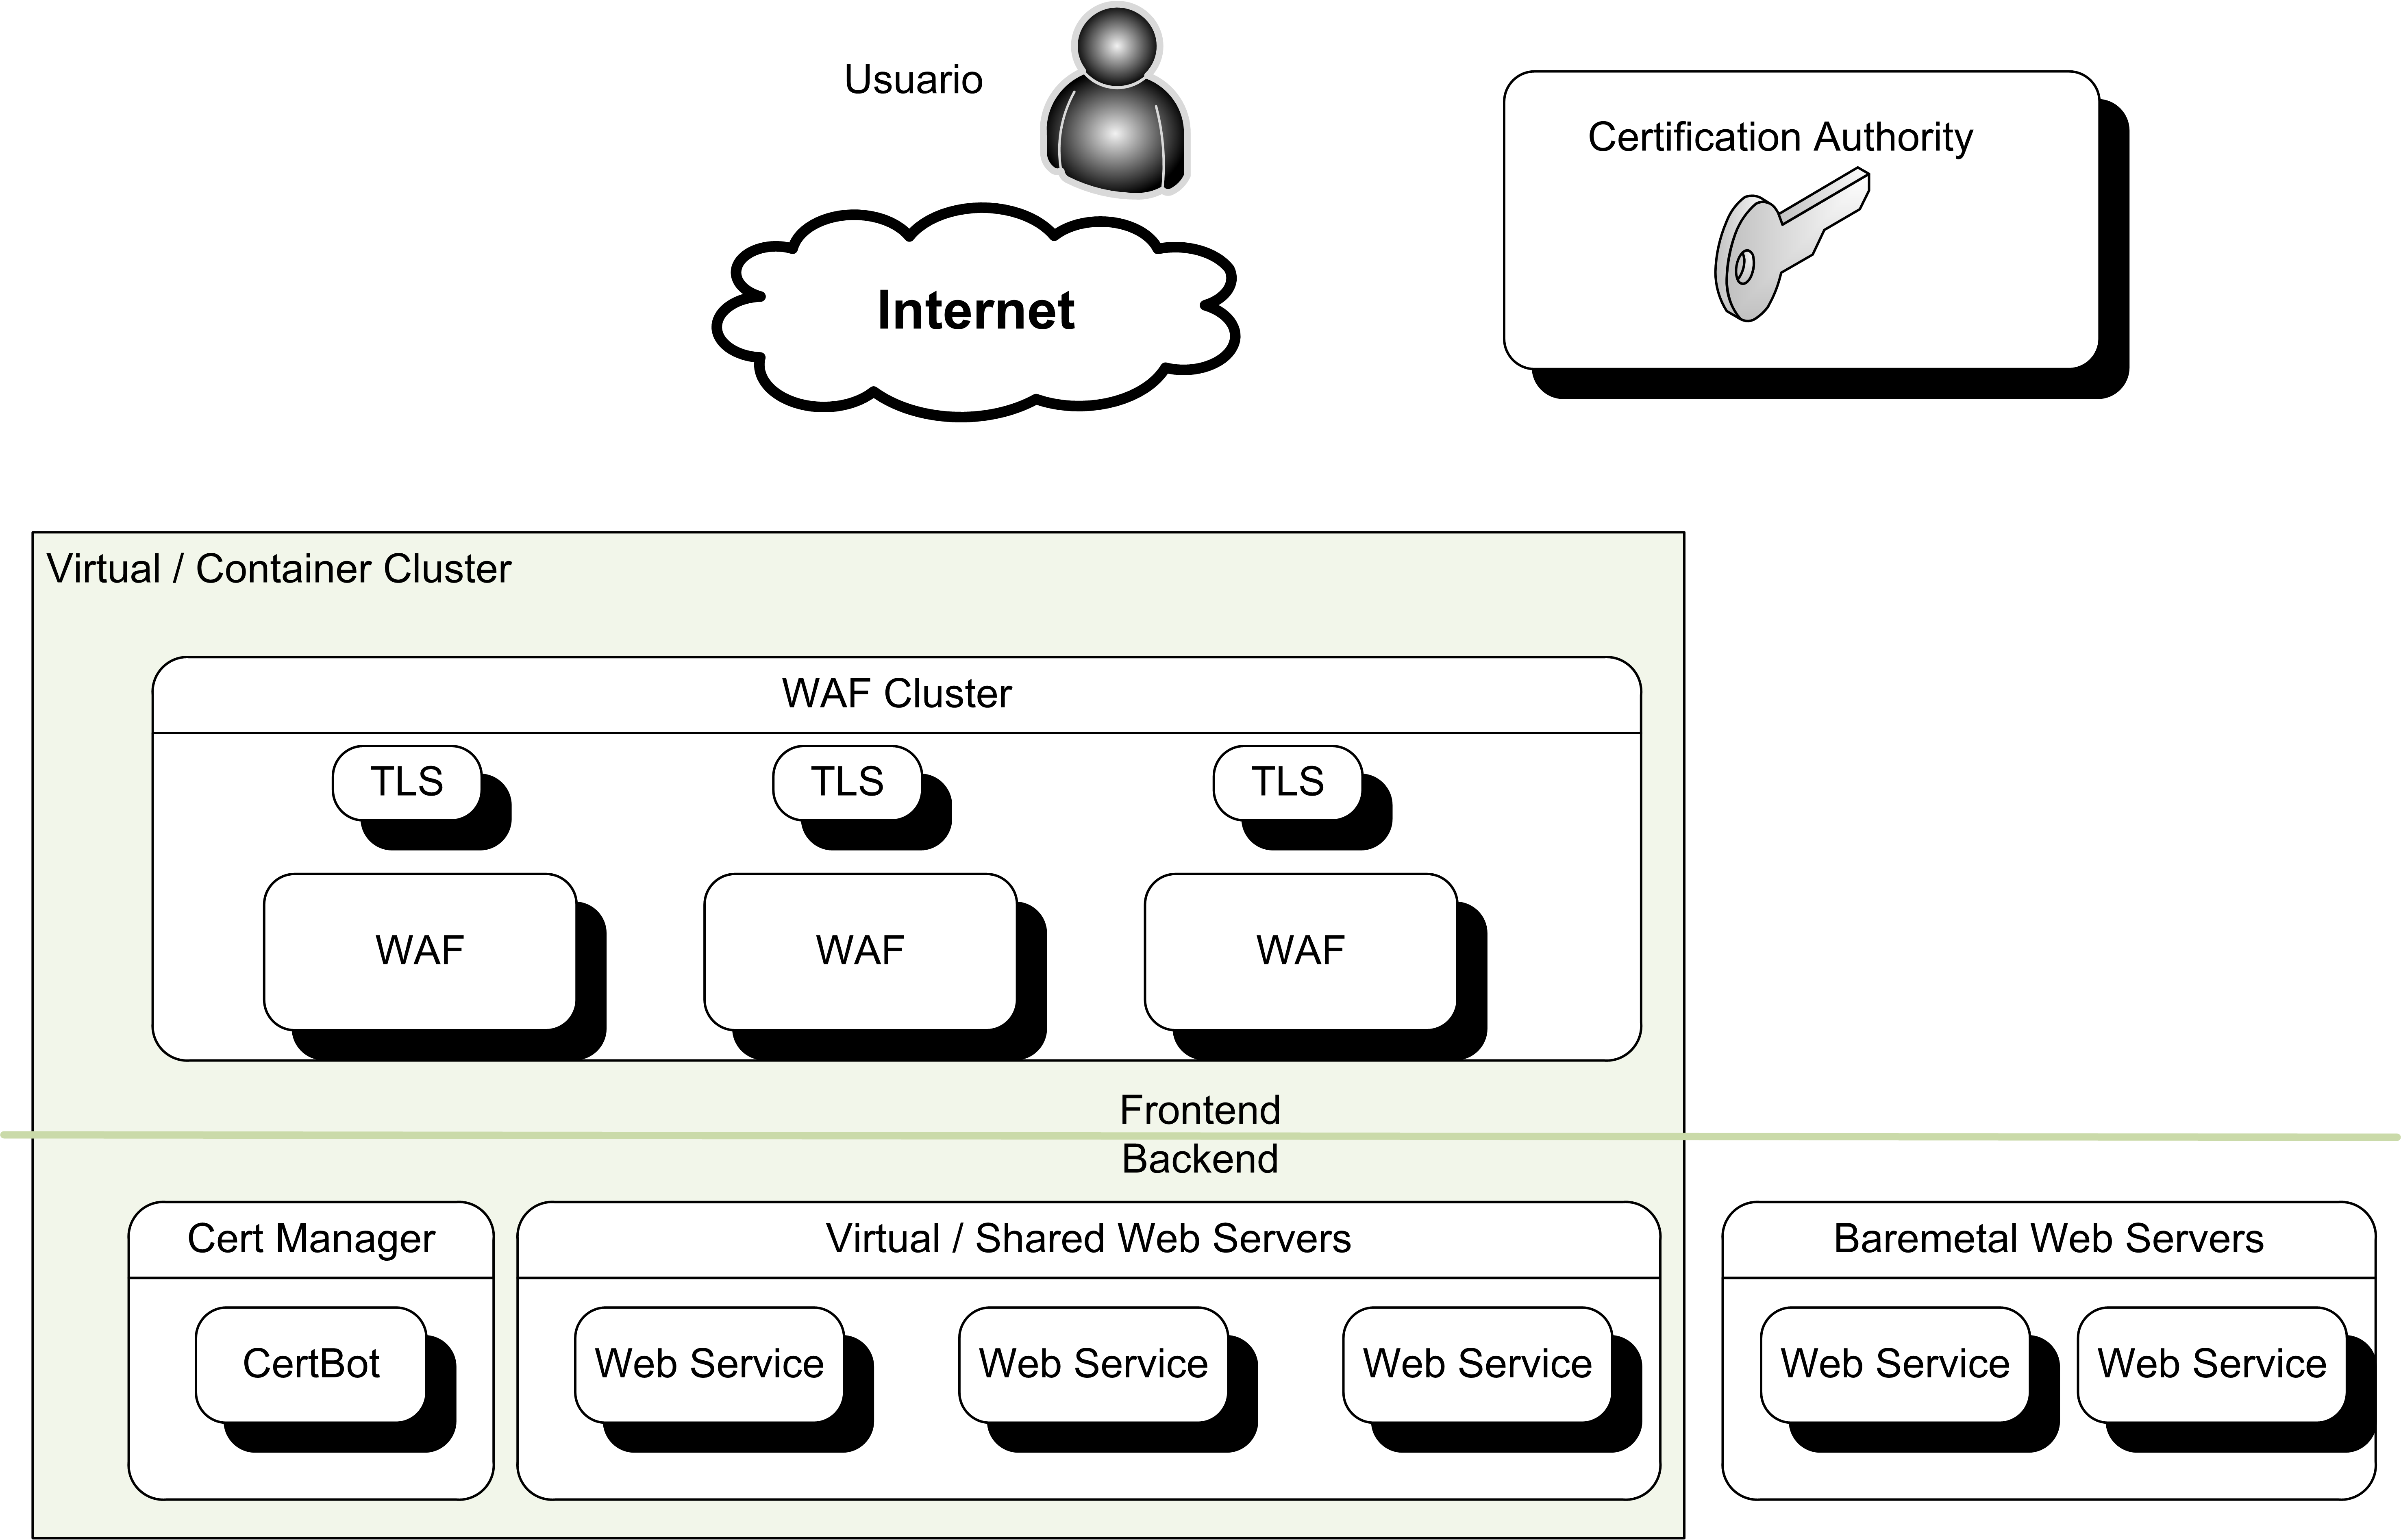
\includegraphics[width=0.9\textwidth]{fig/Diagram_HLD}
    \caption{\small{Diseño a alto nivel de la solución}}
  \end{figure}
\end{frame}

\begin{frame}[shrink]
  \frametitle{Componentes del WAF}
  \begin{figure}
    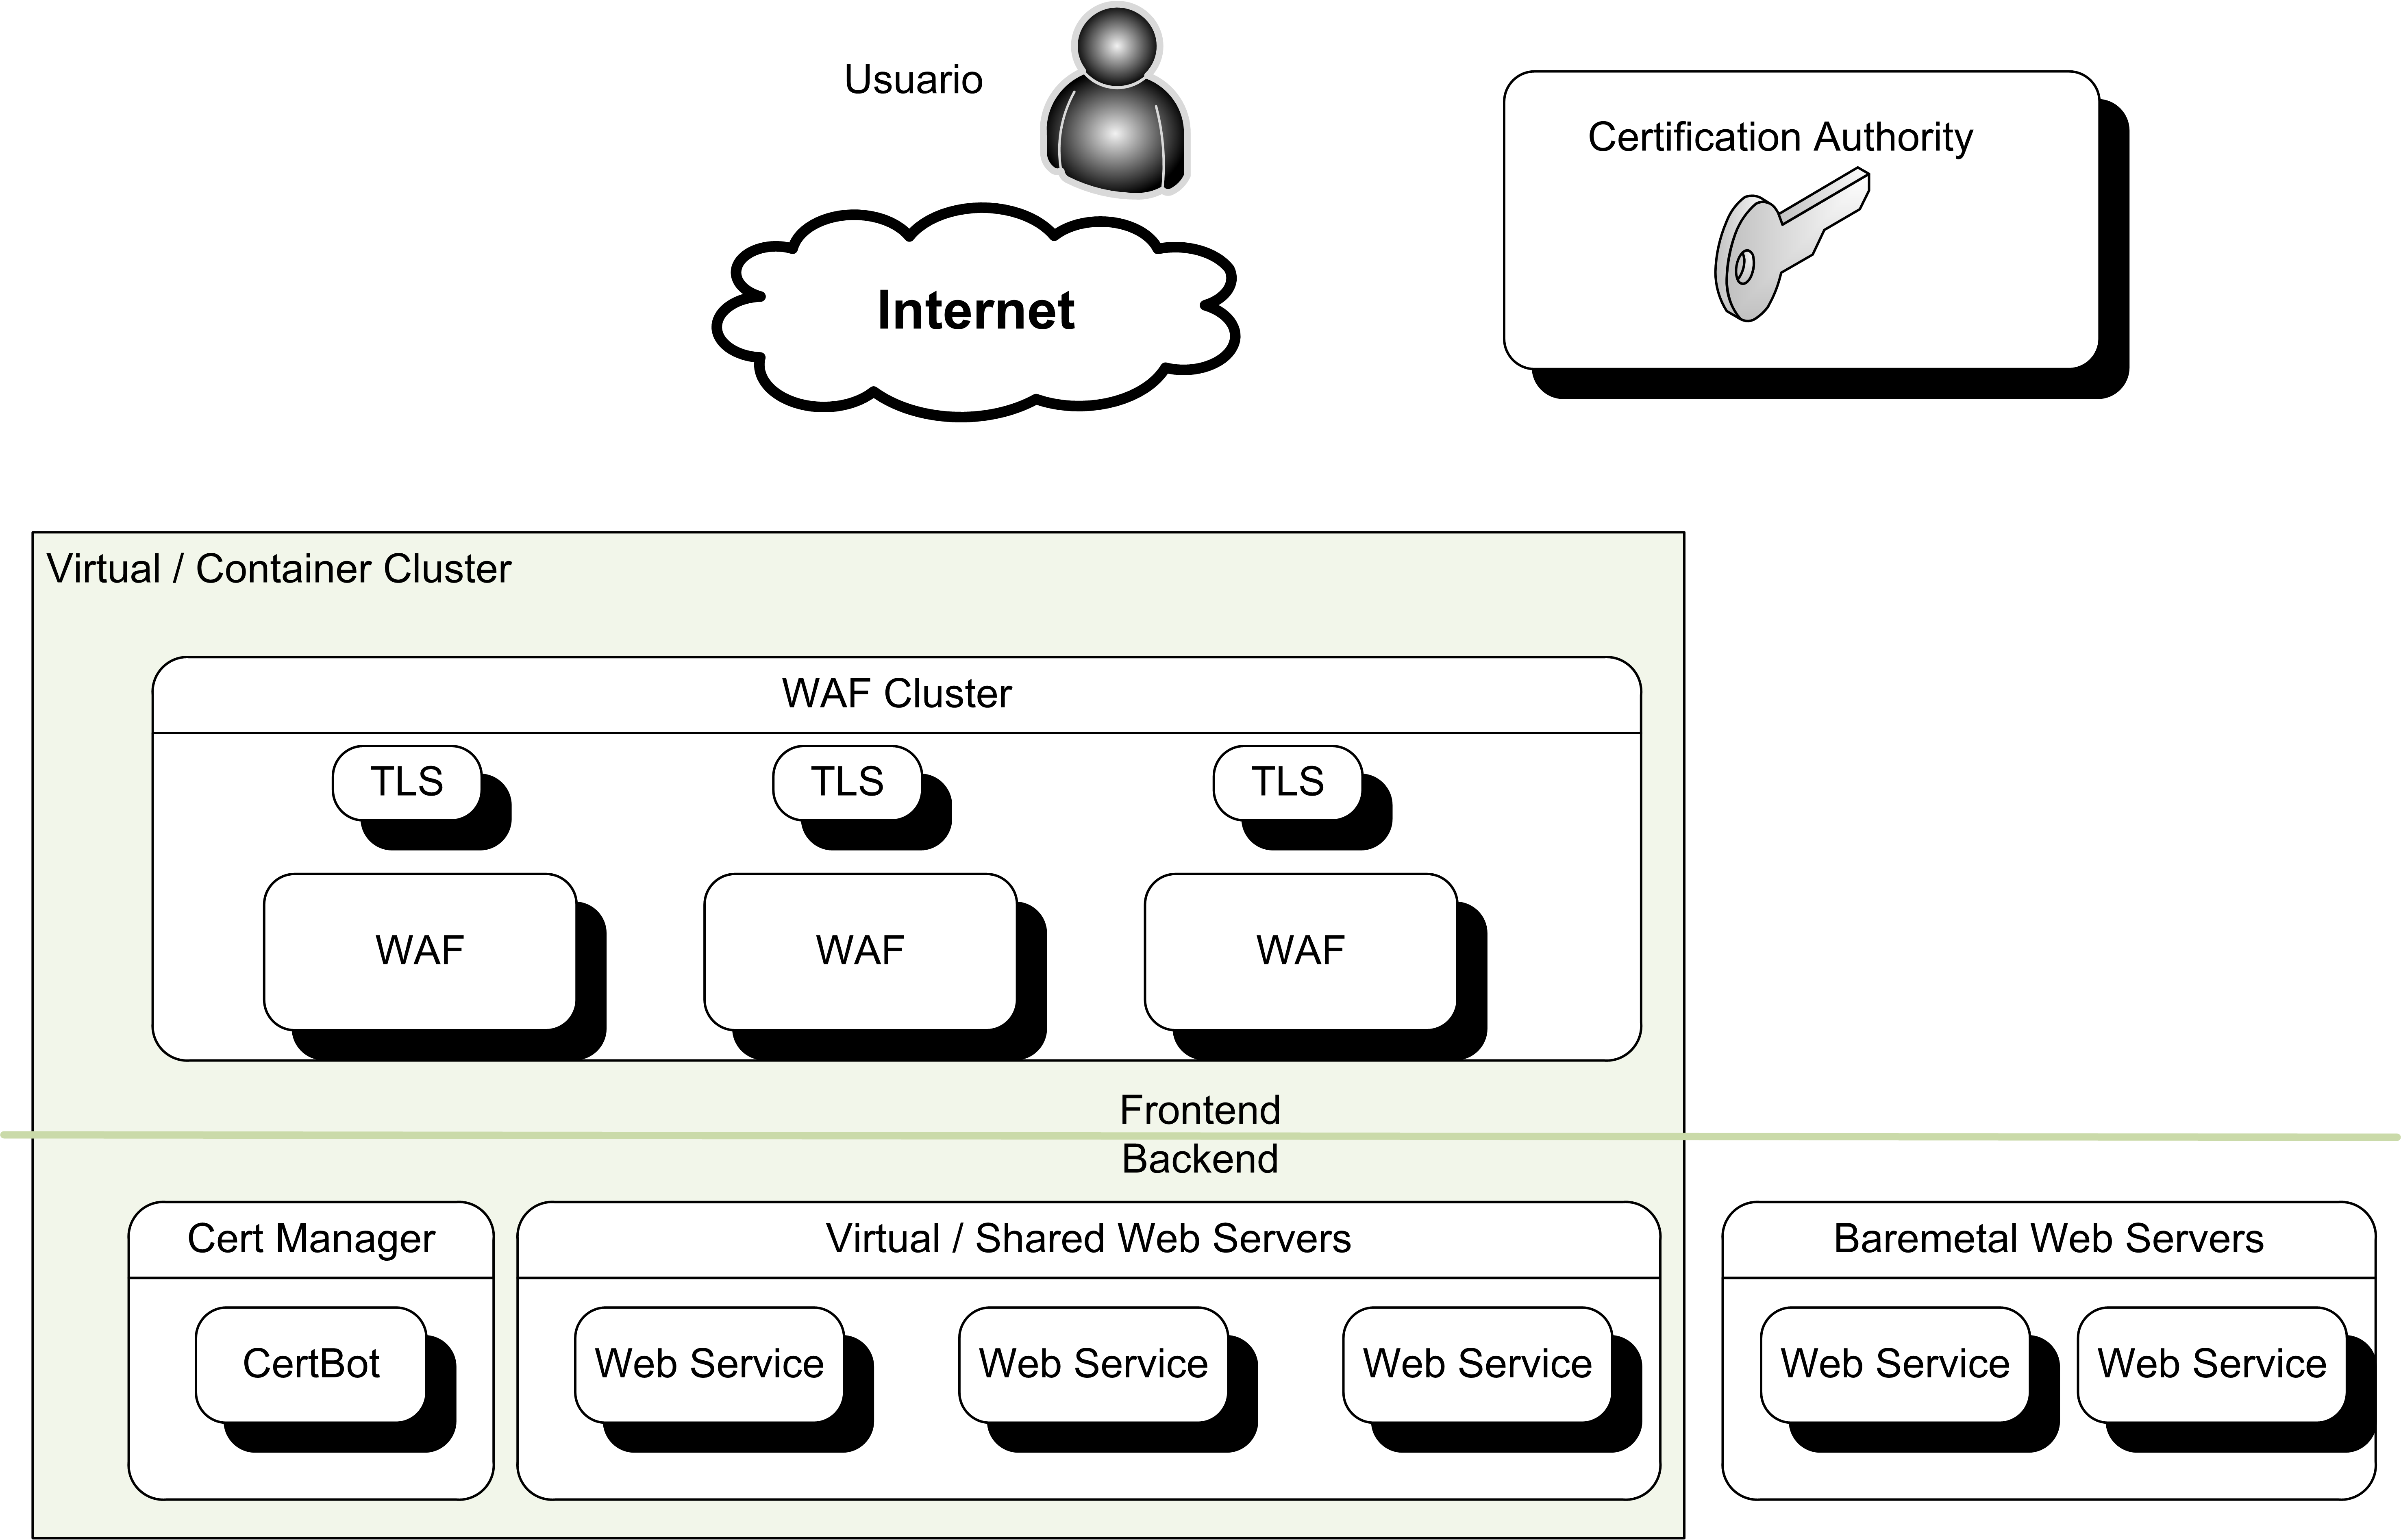
\includegraphics[width=0.9\textwidth]{fig/Diagram_HLD}
    \caption{\small{Diseño a alto nivel de la solución}}
  \end{figure}
\end{frame}

\begin{frame}[shrink]
  \frametitle{Componentes}
  \par Componentes de la solución:
  \begin{tabular}{ l c }
      \acrlong{waf}                                               & \parbox[c]{5em}{
\includegraphics[width=.30\textwidth,height=3cm,keepaspectratio]{fig/ModSecurityLogo}} \\
      Software criptográfico                                      & \parbox[c]{5em}{
\includegraphics[width=.30\textwidth,height=3cm,keepaspectratio]{OpenSSL_logo}} \\
      virtualización (contenedores)                               & \parbox[c]{5em}{
\includegraphics[width=.30\textwidth,height=3cm,keepaspectratio]{fig/DockerLogo}} \\
      Automatización y orquestación.                              & \parbox[c]{5em}{
\includegraphics[width=.30\textwidth,height=3cm,keepaspectratio]{fig/KubernetesLogo}} \\
      Gestión de certificados.                                    & \parbox[c]{5em}{
\includegraphics[width=.30\textwidth,height=3cm,keepaspectratio]{fig/LetsEncryptLogo}} \\
      Políticas y controles de seguridad.                         & \parbox[c]{5em}{
\includegraphics[width=.30\textwidth,height=3cm,keepaspectratio]{fig/OWASPCRSLogo}} \\
    \end{tabular}
\end{frame}


\subsection{Arquitectura}
\begin{frame}[shrink]
  \frametitle{Arquitectura. Gestión de certificados}
  \begin{figure}
    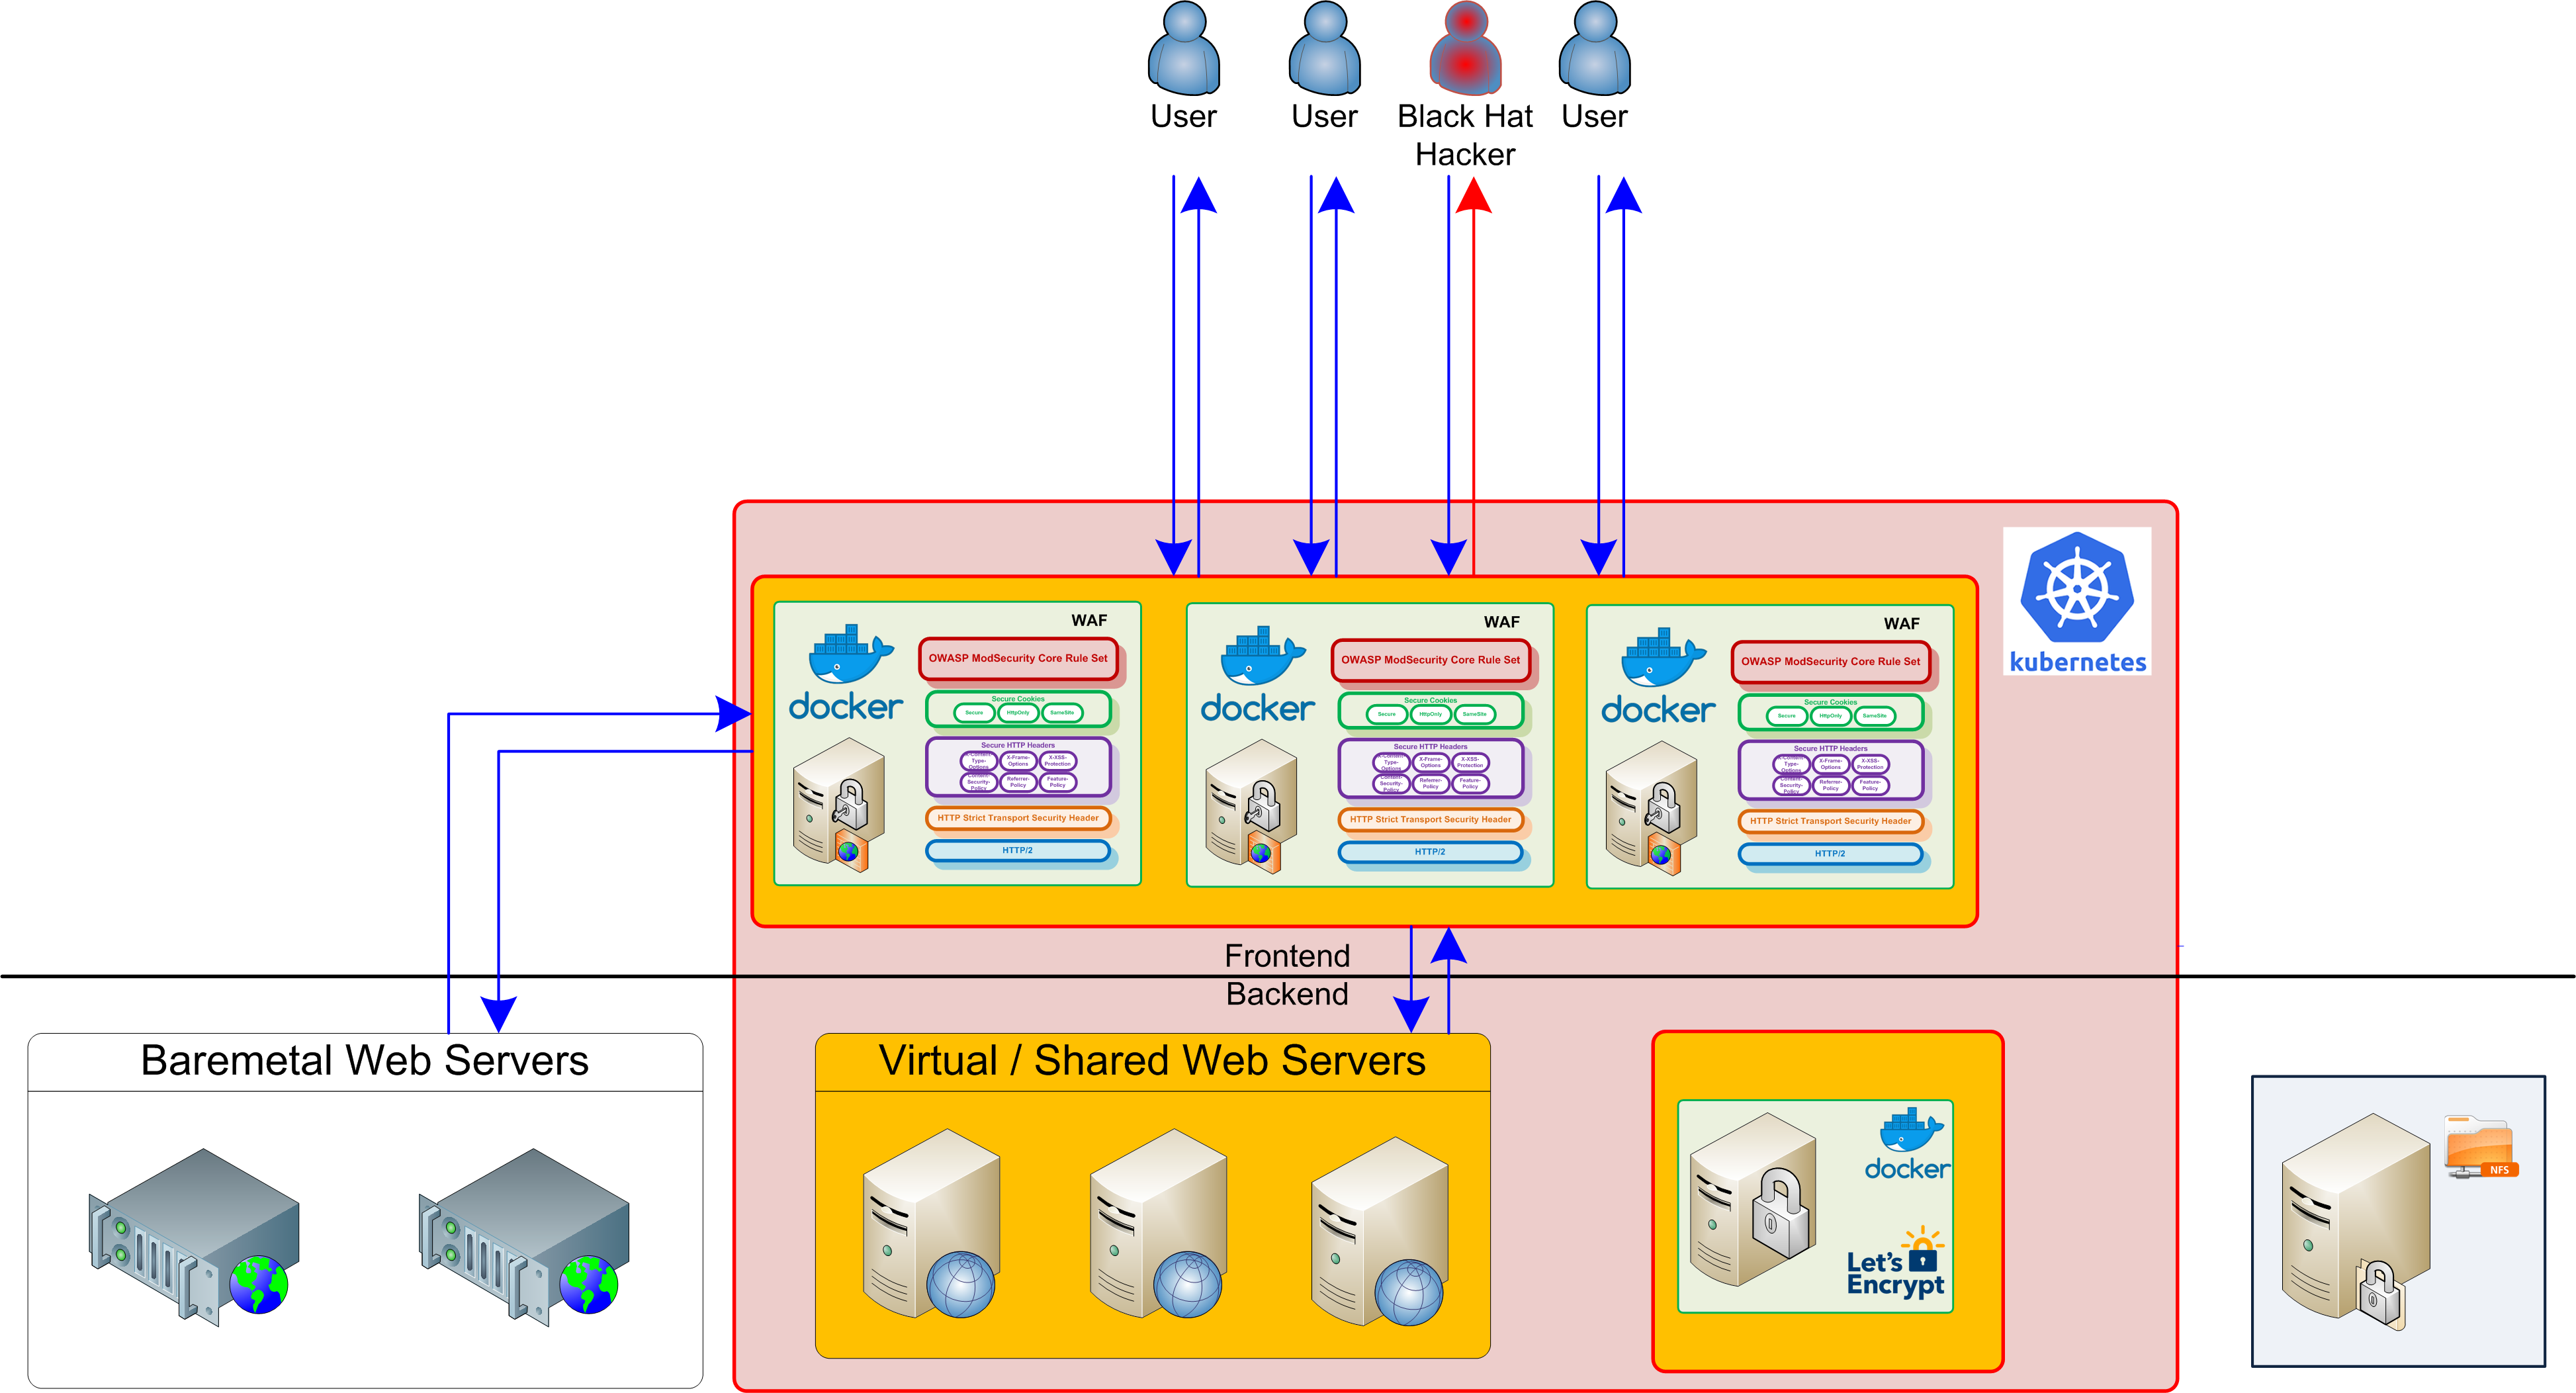
\includegraphics[width=0.9\textwidth]{fig/Diagram_HTTP_Services}
  \end{figure}
\end{frame}

\begin{frame}[shrink]
  \frametitle{Arquitectura. Peticiones HTTP/HTTPS}
  \begin{figure}
    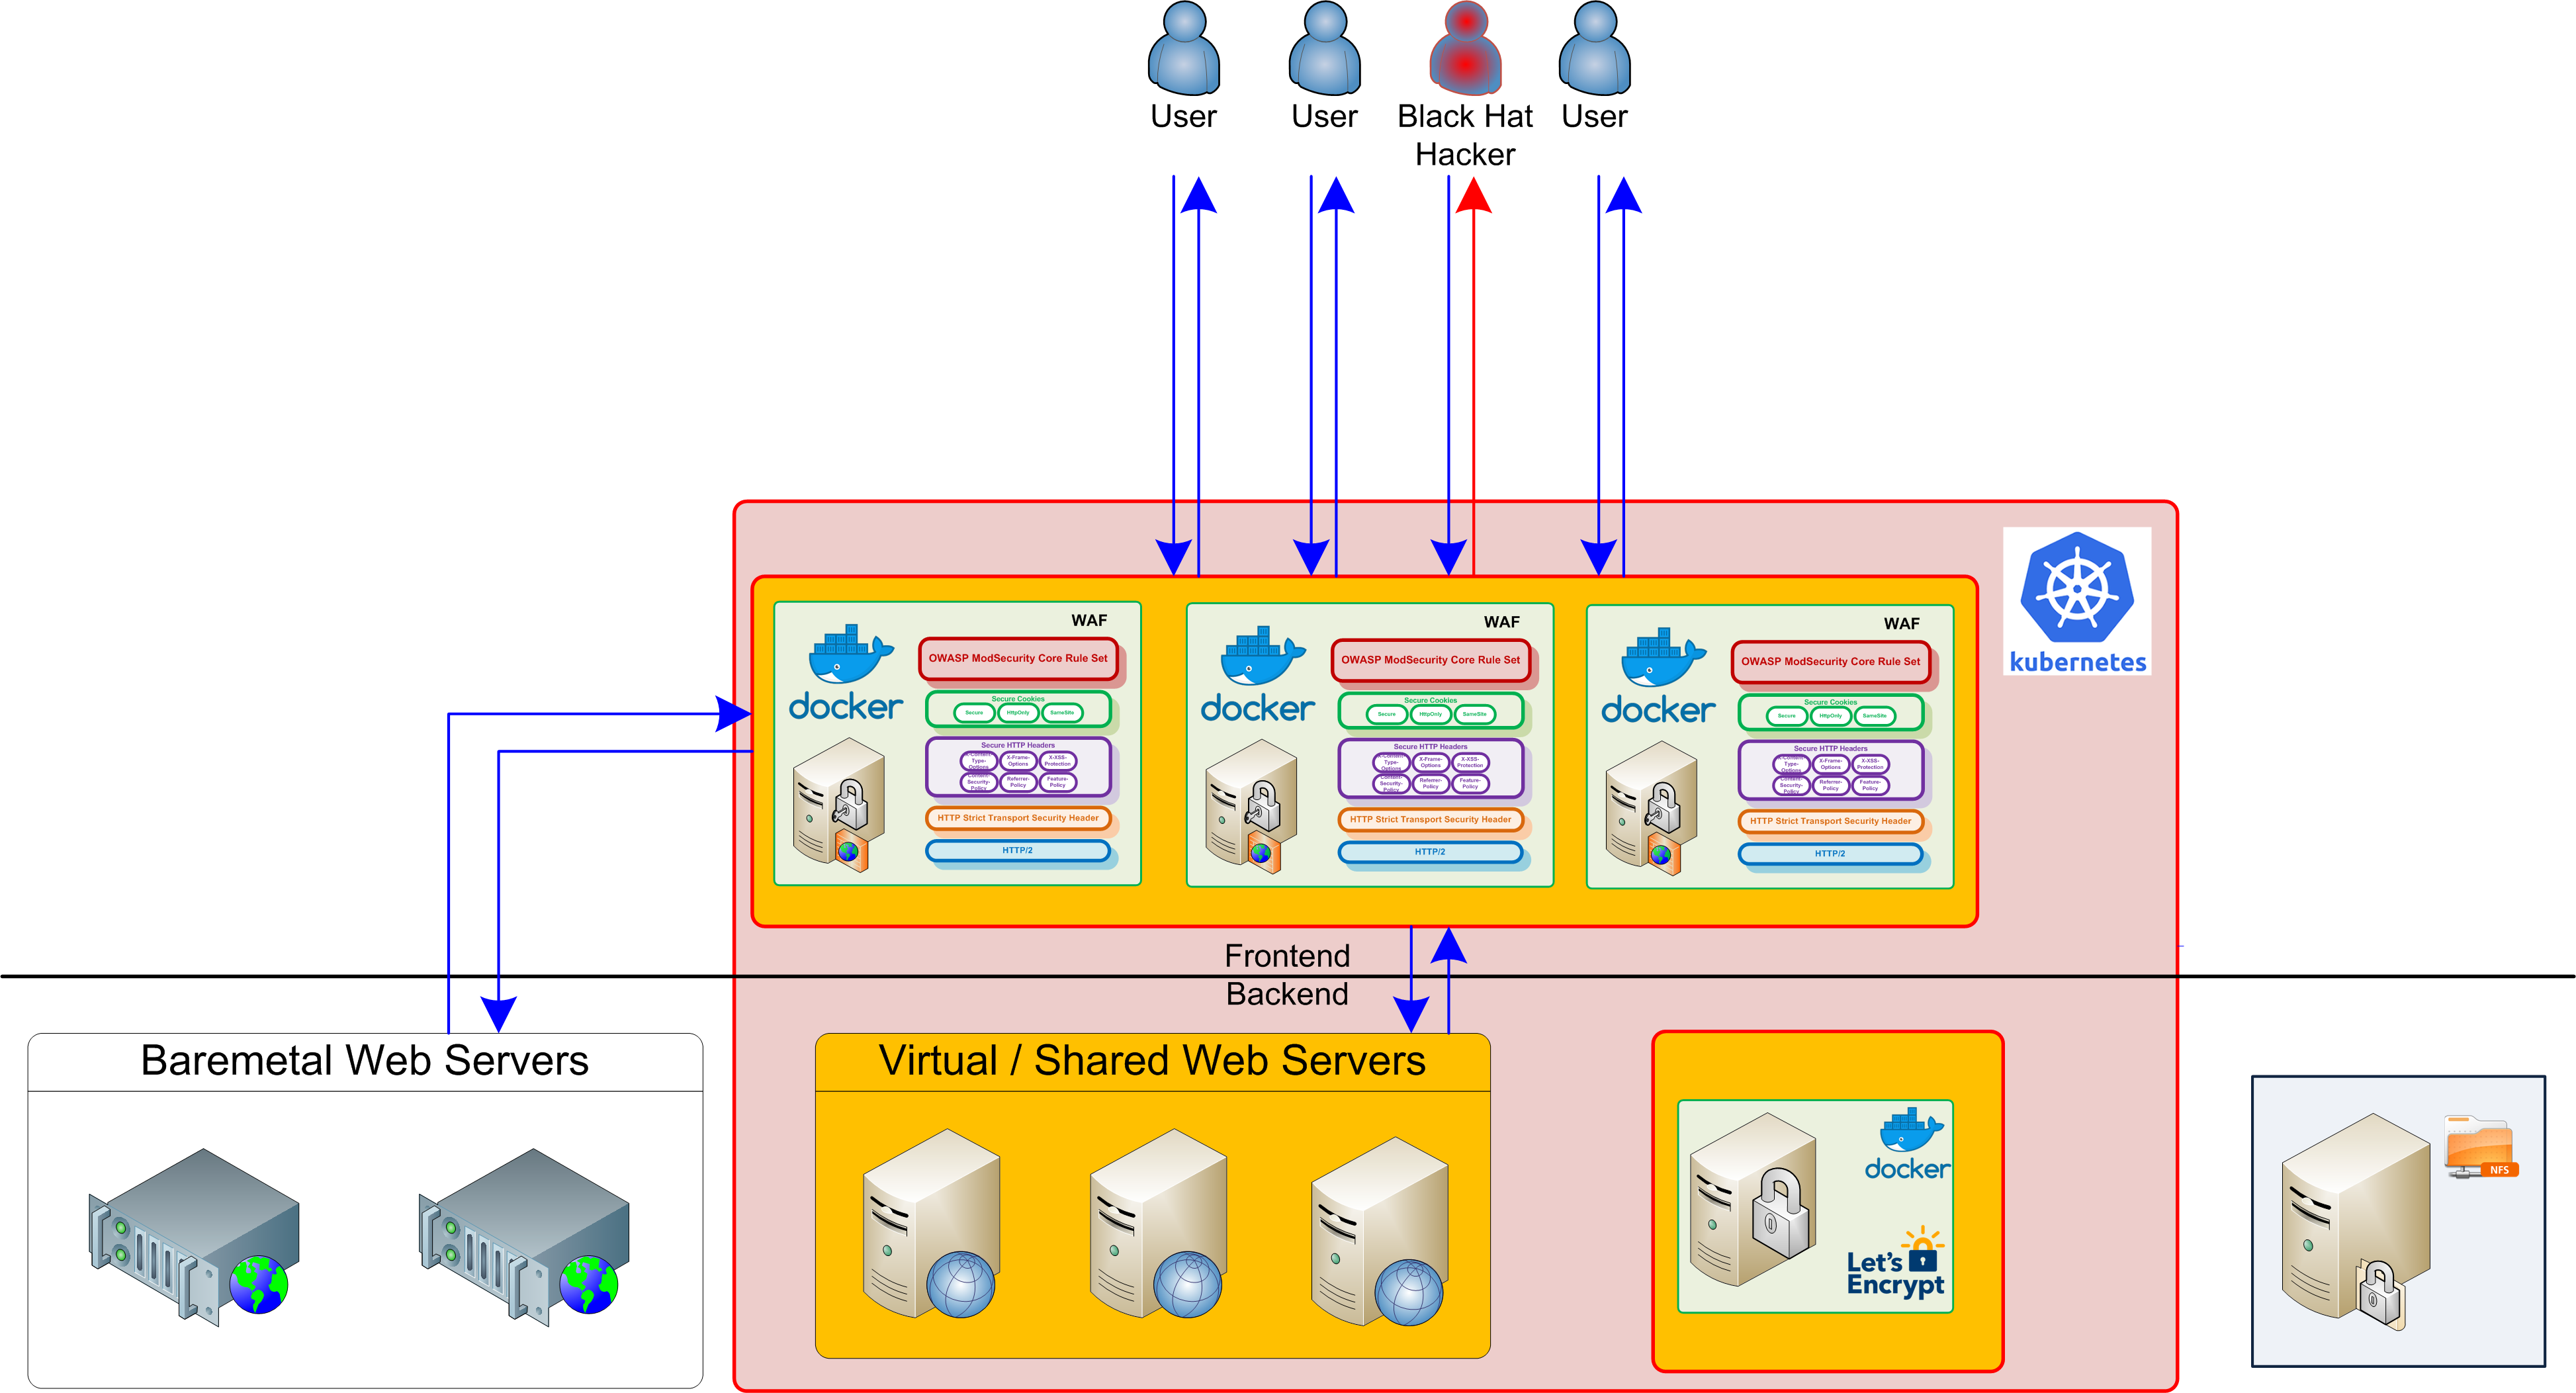
\includegraphics[width=0.9\textwidth]{fig/Diagram_HTTP_Services}
  \end{figure}
\end{frame}


\section{Conclusiones}
\begin{frame}[shrink]
  \frametitle{Conclusiones}
  TODO
\end{frame}


\section{Tests y resultados}
\begin{frame}[shrink]
  \frametitle{Resultados TLS}
  Se ha ejecutado la batería de pruebas proporcionada por Qualys. SSL Labs~\cite{ssllabs} con el siguiente resultado:
  \begin{figure}
    \centering
    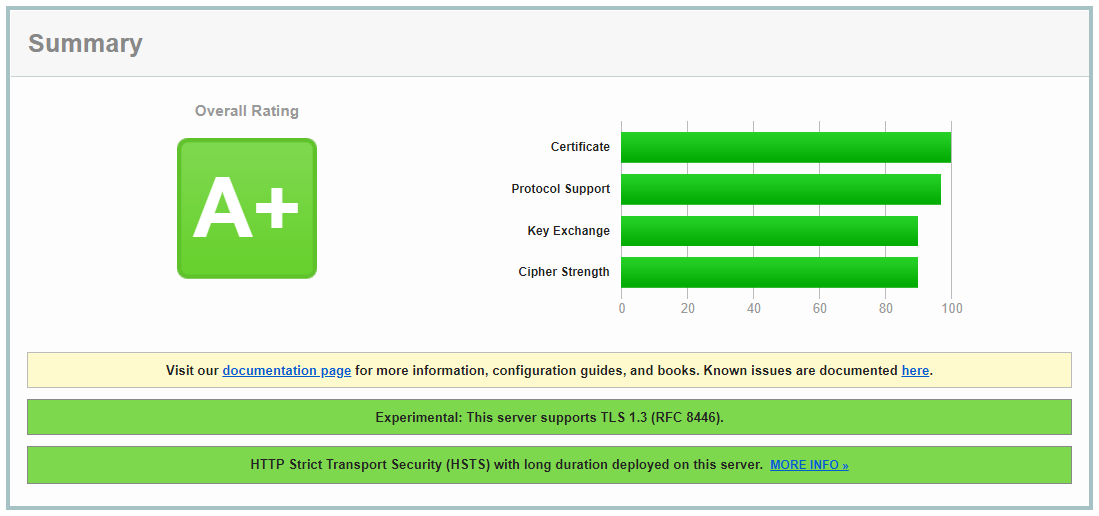
\includegraphics[width=0.8\textwidth]{fig/SSLTLS_Report_Summary}
  \end{figure}
  Entre otros, los test ejecutados incluyen: Configuración TLS, vulnerabilidades TLS y configuración de certificados.
\end{frame}

\begin{frame}[shrink]
  \frametitle{Resultados cabeceras HTTP de seguridad}
  Se ha ejecutado la batería de pruebas proporcionada por Netsparker~\cite{securityheaders} con el siguiente resultado:
  \begin{figure}
    \centering
    
\includegraphics[width=0.9\textwidth]{fig/SecurityHeaders_Report_Summary}
  \end{figure}
  Entre otros, los test ejecutados incluyen: {\em \acrlong{hsts}} (\acrshort{hsts}), {\em X-XSS-Protection}, {\em Content-Security-Policy} o la reciente {\em Feature-Policy}.
\end{frame}




\begin{frame}
  \begin{center}
    \frametitle{Ruegos y preguntas}
    \huge ¿Preguntas?
  \end{center}
\end{frame} 

\end{document}
